
In what follows, we want to solve the system of linear equations
\begin{equation}
{\bm A}\cdot \vec{x} = \vec{b} 
\end{equation}
for the vector $\vec{x}$.
We denote the unique solution of this system by $\vec{x}^\star$.

Note that in some cases the the known $n\times n$ matrix ${\bm A}$ is 
symmetric (i.e., ${\bm A}^T = {\bm A}$), 
positive-definite (i.e. $\vec{x}^T\cdot {\bm A} \cdot \vec{x} > 0$ 
for all non-zero vectors $\vec{x}$ in $\mathbb{R}^n$), 
and real, and $\vec{b}$ is known as well (typically the $\K$ matrix). 


%........................................
\subsubsection{Stationary iterative methods}


Basic examples of stationary iterative methods use a splitting of the matrix ${\bm A}$ such as
\[
{\bm A}={\bm D}+{\bm L}+{\bm U}
\]
where ${\bm D}$ is only the diagonal part of ${\bm A}$, 
${\bm L}$ is the strict lower triangular part of ${\bm A}$ and
${\bm U}$ is the strict upper triangular part of ${\bm A}$.

For instance:
\[
{\bm A}=
\left(
\begin{array}{ccc}
1 & 5 & 8 \\
6 & 4 & 2 \\
-1 & 7 & 5
\end{array}
\right)
\qquad
\Rightarrow
\qquad
{\bm D}=
\left(
\begin{array}{ccc}
1 & 0 & 0 \\
0 & 4 & 0 \\
0 & 0 & 5
\end{array}
\right)
\quad
{\bm L}=
\left(
\begin{array}{ccc}
0 & 0 & 0 \\
6 & 0 & 0 \\
-1 & 7 & 0
\end{array}
\right)
\quad
{\bm U}=
\left(
\begin{array}{ccc}
0 & 5 & 8 \\
0 & 0 & 2 \\
0 & 0 & 0
\end{array}
\right)
\]



\begin{itemize}
\item Jacobi method\footnote{\url{https://en.wikipedia.org/wiki/Jacobi_method}}: 
The solution is then obtained iteratively via

\begin{equation}
{\bm D} \cdot \vec{x}^{{\color{Fuchsia}k+1}} = -({\bm L} + {\bm U}) \cdot \vec{x}^{\color{Fuchsia}k} 
+ \vec{b}
\qquad k=0,1,\dots
\end{equation}
where 
$\vec{x}^{\color{Fuchsia}k}$ is the $k$-th approximation or iteration of $\vec{x}$ and
$\vec{x}^{\color{Fuchsia}0}$ is the initial guess (often taken to be zero).
A sufficient (but not necessary) condition for the method to converge is that the matrix ${\bm A}$ 
is strictly or irreducibly diagonally dominant.

\item Gauss-Seidel method\footnote{\url{https://en.wikipedia.org/wiki/Gauss-Seidel_method}}: 
It is defined by the iteration
\begin{equation}
{\bm L_\star} \cdot \vec{x}^{{\color{Fuchsia}k+1}} = - {\bm U} \cdot \vec{x}^{\color{Fuchsia}k} 
+ \vec{b}
\qquad k=0,1,\dots
\end{equation}
where ${\bm L}_\star = {\bm L}+{\bm U}$.

There is actually a way to make the computation of $\vec{x}^{(k+1)}$ which uses the elements of 
$\vec{x}^{(k+1)}$ that have already been computed, and only the elements of $\vec{x}^{(k)}$ that 
have not been computed in the $k+1$ iteration. 
This means that, unlike the Jacobi method, only one storage vector is required as elements 
can be overwritten as they are computed, which can be advantageous for very large problems. 

Note that Gauss-Seidel is the same as SOR (successive over-relaxation) with $\omega = 1$.

\item Successive over-relaxation method (SOR):
\begin{equation}
({\bm D} + \omega {\bm L}) \cdot \vec{x}^{{\color{Fuchsia}k+1}} 
= - (\omega{\bm U} + (\omega-1) {\bm D}) \cdot \vec{x}^{\color{Fuchsia}k} 
+ \omega \vec{b}
\qquad k=0,1,\dots
\end{equation}


\item Symmetric successive over-relaxation 
(SSOR)\footnote{\url{https://en.wikipedia.org/wiki/Symmetric_successive_over-relaxation}}:
The version of SOR for symmetric matrices ${\bm A}$, in which ${\bm U}={\bm L}^T$ is 
given by the recursion
\begin{equation}
\vec{x}^{{\color{Fuchsia}k+1}} 
=  \vec{x}^{\color{Fuchsia}k} 
-\gamma^k {\bm P}^{-1} ( {\bm A}\cdot \vec{x}^{(k)} -\vec{b})
\qquad k=0,1,\dots
\end{equation}
with 
\[
{\bm P} = \left(\frac{\bm D}{\omega}+{\bm L}\right) \frac{\omega}{2-\omega} {\bm D}^{-1}\cdot
\left(\frac{\bm D}{\omega}+ {\bm L} \right)
\]
with $0<\omega<2$.

%\item Richardson method: 
%\item Damped Jacobi method: 


\end{itemize}

\index{general}{Jacobi solver}
\index{general}{Gauss-Seidel solver}
\index{general}{SOR iterative method}
\index{general}{SSOR iterative method}

\index{general}{GMRES solver}

All these methods can be cast in a more general framework\footnote{
\url{https://en.wikipedia.org/wiki/Iterative_method}}: 
The basic iterative methods work by splitting the matrix A into M-N 
and here the matrix M should be easily invertible. The iterative methods are now defined as 
\begin{equation}
{\bm M} \cdot \vec{x}^{k+1} = {\bm N}\cdot \vec{x}^k + \vec{b}
\end{equation}
with 
\begin{itemize}
\item Richardson method: ${\bm M}=\frac{1}{\omega} {\bm I}$
\item Jacobi method: ${\bm M}={\bm D}$
\item Damped Jacobi method: ${\bm M}=\frac{1}{\omega}{\bm D}$
\item Gauss–Seidel method: ${\bm M}={\bm D} + {\bm L}$
\item Successive over-relaxation method: ${\bm M} = \frac{\bm D}{\omega}+{\bm L}$
\item Symmetric successive over-relaxation:  ${\bm M} = \left(\frac{\bm D}{\omega}+{\bm L}\right) \frac{\omega}{2-\omega} {\bm D}^{-1}\cdot \left(\frac{\bm D}{\omega}+ {\bm L} \right)$
\end{itemize}
and ${\bm N}={\bm M}-{\bm A}$.

%........................................
\subsubsection{Krylov subspace methods}

\index{general}{CG solver}
\begin{itemize}
\item {\color{purple} Conjugate Gradient}
\footnote{\url{https://en.wikipedia.org/wiki/Conjugate_gradient_method}} 

It was first proposed by Hestenes and Stiefel in 1952 \cite{hest52}.
The method solves an SPD system ${\bm A}\cdot \vec{x} = \vec{b}$ of size $n$.
In theory (i.e. exact arithmetic) it does so in $n$ iterations.
Each iteration requires a few inner products in $\mathbb{R}^n$ and one matrix-vector multiplication.
With roundoff error, CG can work poorly (or not at all), but for some 
${\bm A}$ (and $\vec{b}$), can get good approximate solution in $<<n$ iterations.

As an iterative method, the conjugate gradient method monotonically (in the energy norm) 
improves approximations $\vec{x}_k$ to the exact solution and
may reach the required tolerance after a relatively small (compared to the problem size) number 
of iterations. The improvement is typically linear and its speed is determined by the 
condition number $\kappa({\bm A})$ of the system matrix ${\bm A}$: 
the larger $\kappa({\bm A})$ is, the slower the improvement.

If $\kappa({\bm A})$ is large, preconditioning is commonly used to replace the 
original system ${\bm A} \cdot \vec{x}-\vec{b}=\vec{0}$ 
with ${\bm M}^{-1}\cdot ({\bm A} \cdot \vec{x}-\vec{b})=\vec{0}$ 
such that $\kappa({\bm M}^{-1}\cdot {\bm A})$ 
is smaller than $\kappa({\bm A})$. 

The resulting method is called the Preconditioned Conjugate Gradient method (PCG).
An extreme case of preconditioner is ${\bm M}={\bm A}^{-1}$ but it is a silly case
since applying the preconditioner is as difficult as solving the system in the 
first place.
In the end the goal is to find a matrix ${\bm M}$ that is cheap to multiply, 
and is an approximate inverse of ${\bm A}$ 
(or at least has a more clustered spectrum than ${\bm A}$).

\begin{center}
\frame{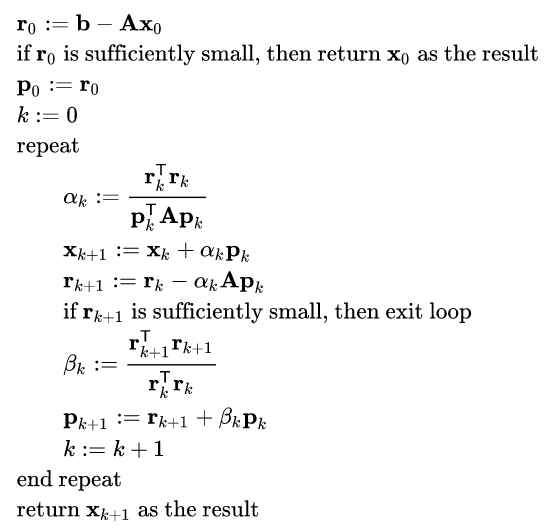
\includegraphics[height=5.6cm]{images/solvers/cgwiki}}
\frame{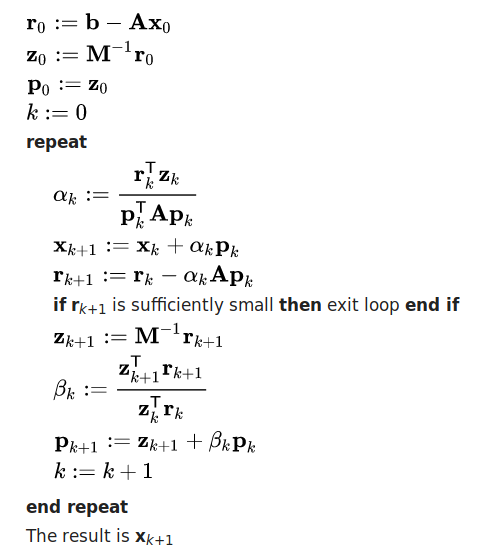
\includegraphics[height=5.6cm]{images/solvers/pcgwiki}}
\frame{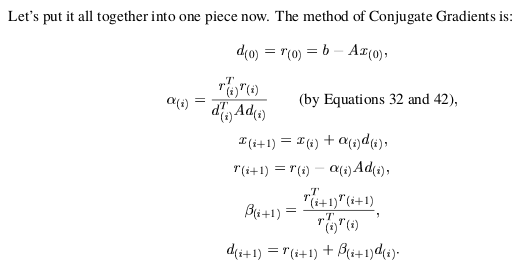
\includegraphics[height=5.6cm]{images/solvers/shew94}}\\
{\captionfont Top: algorithms as obtained from Wikipedia (Left: CG; Right: PCG);
Bottom: algorithm from Shewchuk (1994) \cite{shew94}.}
\end{center}

Also available on Wikipedia is a (naive) MATLAB implementation of the CG algorithm:
\begin{center}
\frame{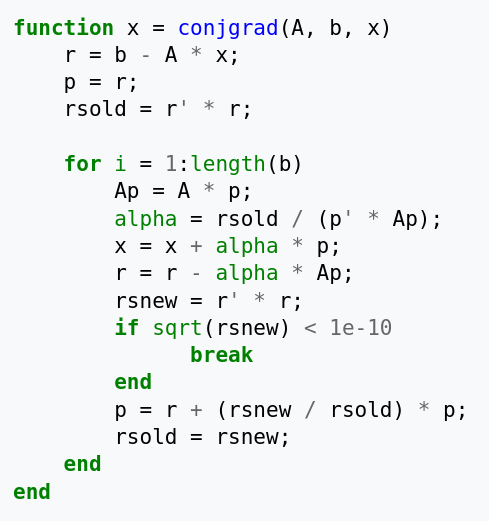
\includegraphics[height=6cm]{images/solvers/cgwiki2}}
\end{center}
We see that its implementation is actually rather simple and straightforward!

\Literature: Shewchuk, An Introduction to the Conjugate 
Gradient Method Without the Agonizing Pain \cite{shew94}

The CG and PCG algorithms are used in Section~\ref{ss:schurpcg}.
It is implemented in \stone~15,16,82.








\index{general}{BiCG solver}
\item Biconjugate Gradient method
\footnote{\url{https://en.wikipedia.org/wiki/Biconjugate_gradient_method}}
\item Biconjugate Gradient stabilised method
\footnote{\url{https://en.wikipedia.org/wiki/Biconjugate_gradient_stabilized_method}}
\item MINRES: For iterative solution of symmetric systems Ax = b, the conjugate gradient method
(CG) is commonly used when A is positive definite, while the minimum residual method (MINRES)
is typically reserved for indefinite systems.


\item Generalized minimal residual method (GMRES)
\footnote{\url{https://en.wikipedia.org/wiki/Generalized_minimal_residual_method}}
\end{itemize}





